%%% LaTeX Template: Two column assignment for BRSU
%%% Based on two column article from: http://www.howtotex.com/
%%% Preamble
\documentclass[	DIV=calc,%
				paper=a4,%
				fontsize=11pt,%
				twocolumn]{scrartcl}	 % KOMA-article class

\usepackage{lipsum}	% Package to create dummy text
\usepackage{blindtext}
\usepackage[english]{babel}	                          % English language/hyphenation
\usepackage[protrusion=true,expansion=true]{microtype} % Better typography
\usepackage{amsmath,amsfonts,amsthm}					 % Math packages
\usepackage[pdftex]{graphicx}	                          % Enable pdflatex
\usepackage[svgnames]{xcolor}	                          % Enabling colors by their 'svgnames'
\usepackage[hang, small,labelfont=bf,up,textfont=it,up]{caption} % Custom captions under/above floats
\usepackage{epstopdf}	 % Converts .eps to .pdf
\usepackage{subfig}	     % Subfigures
\usepackage{booktabs}	 % Nicer tables
\usepackage{fix-cm}       % Custom fontsizes
\usepackage{listings}
\usepackage{soul}

%%% Custom sectioning (sectsty package)
\usepackage{sectsty}	 % Custom sectioning (see below)
\allsectionsfont{%% Change font of al section commands
	\usefont{OT1}{phv}{b}{n}%% bch-b-n: CharterBT-Bold font
	}

\sectionfont{%% Change font of \section command
	\usefont{OT1}{phv}{b}{n}%% bch-b-n: CharterBT-Bold font
	}


\definecolor{brsugrey}{rgb}{0.9, 0.9, 0.9}
\definecolor{brsublue}{rgb}{0, 0.594, 0.949}


\newcommand{\upperRomannumeral}[1]{\uppercase\expandafter{\romannumeral#1}}

%%% Headers and footers
\usepackage{fancyhdr} % Needed to define custom headers/footers
	\pagestyle{fancy} % Enabling the custom headers/footers
\usepackage{lastpage}	

% Header (empty)
\lhead{}
\chead{}
\rhead{}
% Footer (you may change this to your own needs)
\lfoot{\footnotesize 
\texttt{LAA} % Set to the course abbreviation 
\textbullet ~ Hagg % Set to your name
\textbullet ~ Assignment \upperRomannumeral{2}} % Set the assignment number
\cfoot{}
\rfoot{\footnotesize page \thepage\ of \pageref{LastPage}}	% "Page 1 of 2"
\renewcommand{\headrulewidth}{0.0pt}
\renewcommand{\footrulewidth}{0.4pt}



%%% Creating an initial of the very first character of the content
\usepackage{lettrine}
\newcommand{\initial}[1]{%
     \lettrine[lines=3,lhang=0.3,nindent=0em]{
     				\color{brsublue}
     				{\textsf{#1}}}{}}

%%% Title, author and date metadata
\usepackage{titling}	% For custom titles

\newcommand{\HorRule}{\color{brsublue}% Creating a horizontal rule
					 \rule{\linewidth}{1pt}%
					 \color{black}
					 }

\pretitle{\vspace{-30pt} \begin{flushleft} \HorRule 
				\fontsize{25}{25} \usefont{OT1}{phv}{b}{n} \color{gray} \selectfont 
				}
\title{Learning and Adaptivity
\\ Assignment ~\upperRomannumeral{1}}% Title of your article goes here
\posttitle{\par\end{flushleft}\vskip 0.5em}

\preauthor{\begin{flushleft}
\large \lineskip 0.25em \usefont{OT1}{phv}{b}{sl} \color{brsublue}}
\author{Alexander Hagg, Adam Gaier }	% Author name goes here
\postauthor{\footnotesize \usefont{OT1}{phv}{m}{sl} \color{Black} 
BRS University of Applied Sciences % Institution of author
\\email: alexander.hagg@smail.inf.h-brs.de ~github: @alexander-hagg
\par\end{flushleft}\HorRule}

\date{\today} 

%%% Begin document
\begin{document}
\maketitle
\thispagestyle{fancy} % Enabling the custom headers/footers for the first page 
% The first character should be within \initial{}
\initial{A}\textbf{ one paragraph abstract of the topic which the assignment covers can go here. Try to summarize the topic in five sentences. This should be considered preparation for the exam were you are expected to talk about the subject in your own words.}


\setcounter{section}{5}
\section{Decision Tree Learning}
\subsection{Simple Prediction}

\blindenumerate[4]

\subsection{Scalability}

\blindlist{enumerate}[2]

\subsection{Noise}

\blindlist{enumerate}[4]

\vfill

\section*{Conclusion}

After doing the assignment, and playing with machine learning we want to get a few of your thoughts. 

Where the assignment abstract began as a general summary of the topic, which you can use for your exam studying- the conclusion should be more specific to the course content. Feedback can be included here. Also I would like to know if there are any issues with the assignments. If you felt the assignment was \textbf{\hl{stupid}}, please write your arguments for here.  If you really want to get our attention, \hl{you should highlight your text} 

We want to make this course as applicable and useful as possible, and this can only be done with useful and continuous feedback. We are actively investigating the best tools for teaching machine learning. 

\section*{Sources}
Sources are expected. If you follow a tutorial online, used a stack overflow answer or github repo then list it here. Getting caught will result in trouble.
\blindenumerate[3]

\newpage

\onecolumn
\section*{Appendix A: Code}

Once you've answered the assignment questions please include only relevant code snippets in the appendix. You're expected to submit full working source code with the assignments in a subdirectories of your zipped assignment folder. The bellow snippets are not really relevant, but I can't give out assignment solutions here. 

\HorRule

\lstinputlisting[language=Python, numbers=left, firstline=20, 
				lastline=40, frame=L, title=\lstname]{code/letters_ml.py}

\HorRule

\lstinputlisting[language=Python, numbers=left, firstline=20, 
				lastline=35, frame=L, title=\lstname]{code/zoo_ml.py}

\newpage


\section*{Appendix B: Results}

Your results should be written in your assignment answers Images, Figures etc. should be included in this appendix. Use \LaTeX to properly refer to the correct figure if needed, same goes for code snippets. The assignment answers should discuss the results, we are interested in assessing your knowledge. If you're told to generate 10 figures from the same data set, you need to include all the figures in sub directories of your assignment zip folder, but you should only include in the appendix as many figures as needed to back up your answer. 

\HorRule

\begin{figure}[h]
  \centering
  \caption{A decision tree of zoo animals \\ Include the filename, and try to pick readable graphics}
  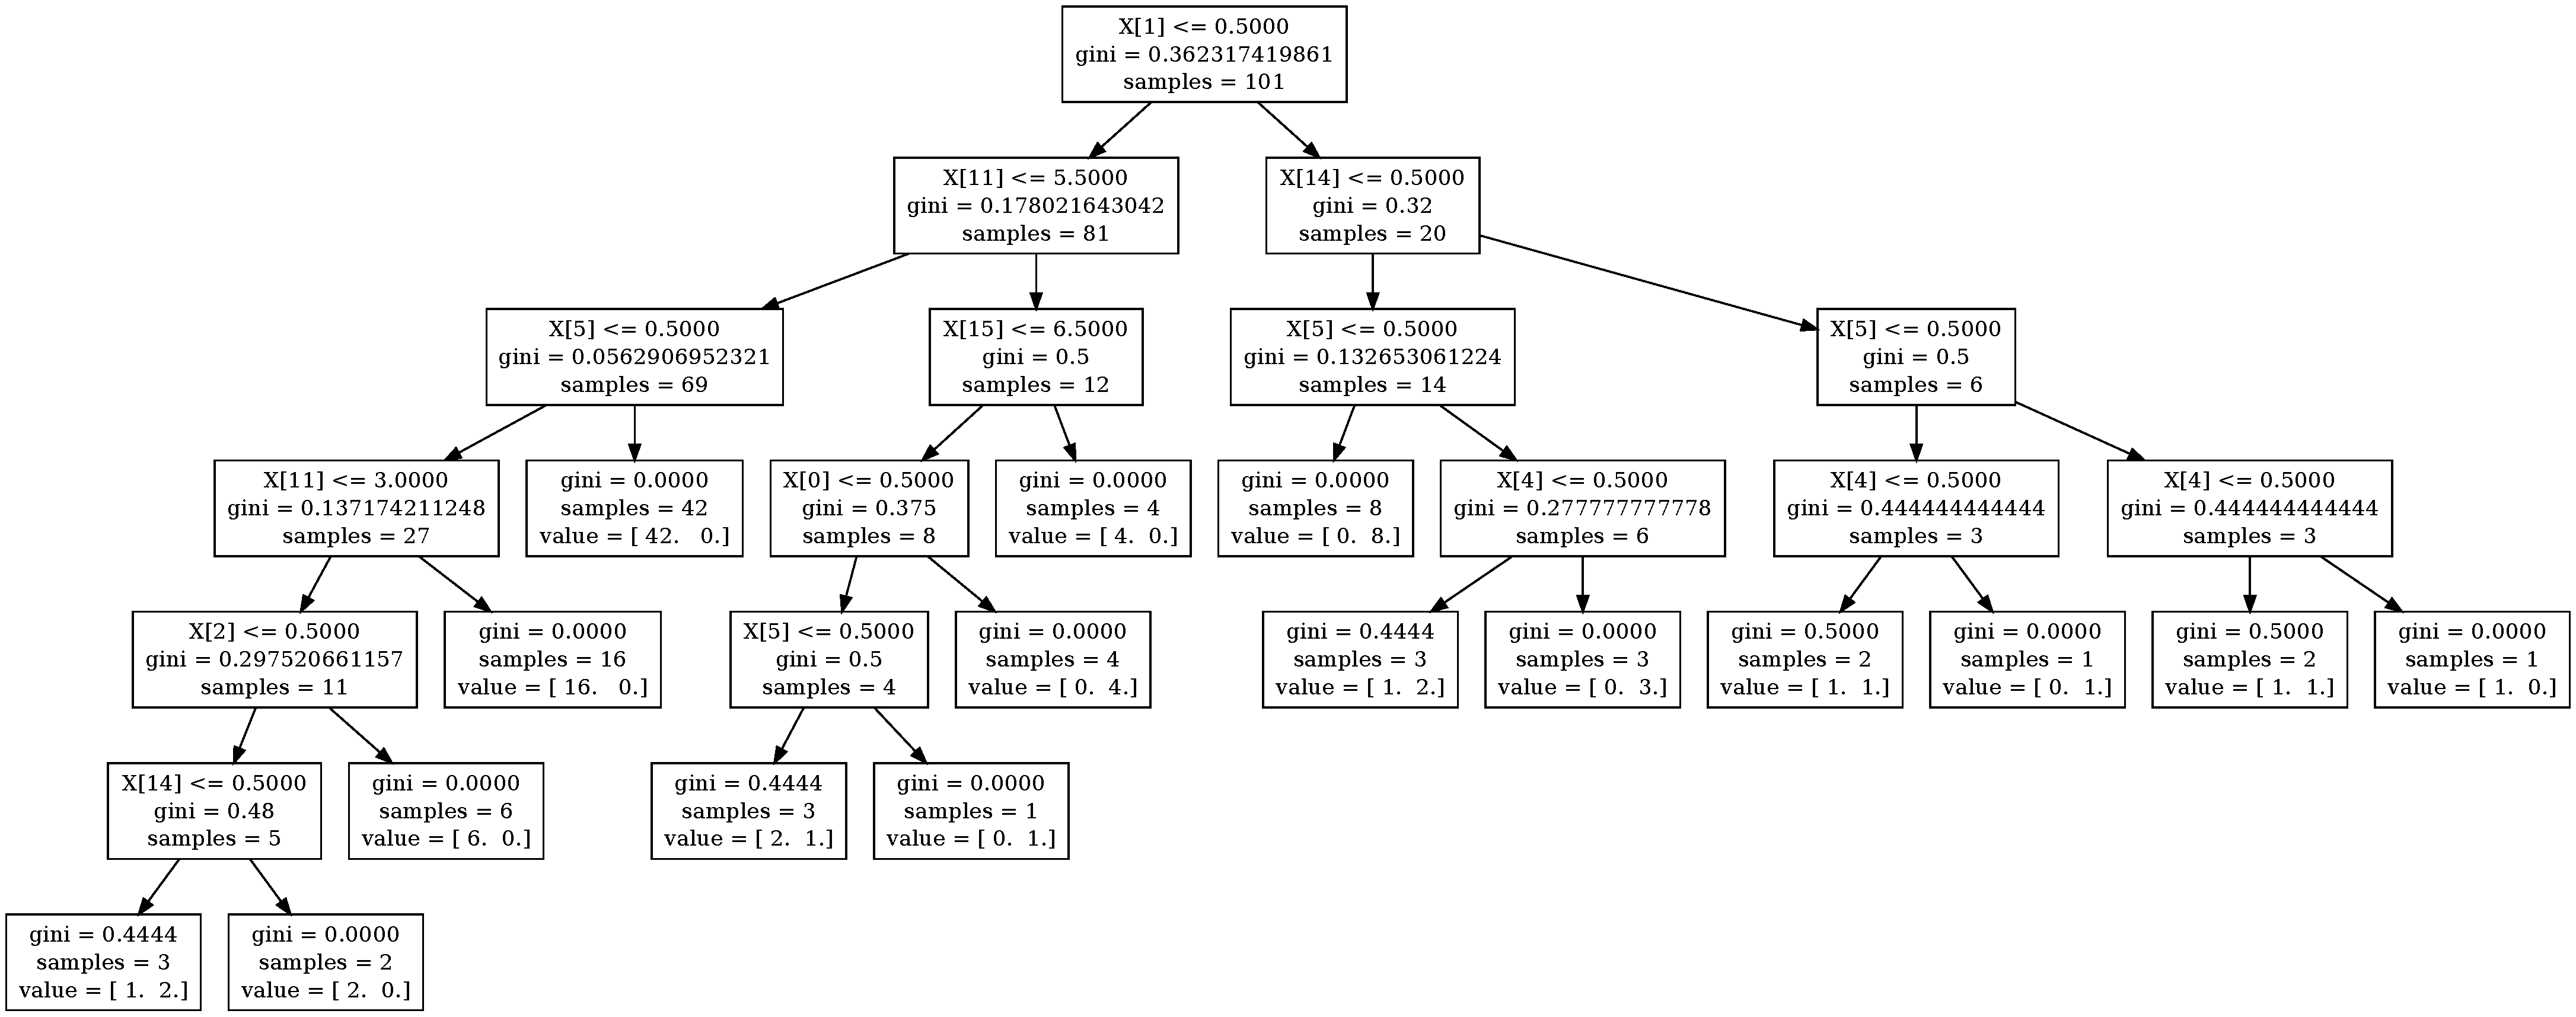
\includegraphics[width=1\textwidth]{./data/q_1_c}
\end{figure}

\end{document}